\RequirePackage[l2tabu, orthodox]{nag}
\documentclass[11pt, oneside]{article}
\usepackage{geometry}
\geometry{letterpaper}
\usepackage{graphicx}

\usepackage{amssymb}
\usepackage{amsmath}

\usepackage{minted}
\usepackage{hyperref}

\usepackage{color}

\usepackage{graphicx}

\usepackage[english]{babel}
\usepackage[utf8]{inputenc}
\usepackage[T1]{fontenc}
\usepackage{lmodern}

\usepackage{microtype}

\newcommand{\blue}[1]{\textcolor{blue}{#1}}
\newcommand{\red}[1]{\textcolor{red}{#1}}
\newcommand{\green}[1]{\textcolor{green}{#1}}
\newcommand{\pe}[1]{\blue{PE: #1}}

\newenvironment{polynomial}
  {\par\vspace{\abovedisplayskip}%
   \setlength{\leftskip}{\parindent}%
   \setlength{\rightskip}{\leftskip}%
   \medmuskip=4mu plus 2mu minus 2mu
   \binoppenalty=0
   \noindent$\displaystyle}
  {$\par\vspace{\belowdisplayskip}}



\newcommand{\ans}[1]{\blue{
\begin{polynomial}
#1
\end{polynomial}
}}


\newcommand{\vect}[1]{\vec{\lowercase{#1}}}

\title{Homework \#2}
\author{Haylee Crane \\
Paul English}

\begin{document}
\maketitle

\begin{enumerate}

\item \textbf{Taylor Series:} Let $f(x) = e^x$ and $g(x) = \ln(x + 1)$, and let $p_n$ and $q_n$ be the Taylor polynomials of degree $n$ for $f$ and $g$, repectively, about $x_0 = 0$.

Plot the graphs of $f$, $g$, $p_n$ and $q_n$, for some small values of $n$, and comment on your results. Discuss in particular how well $f$ and $g$ are approximated by their Taylor polynomials. Explain your observations in terms of a suitable expression for the error in the approximation.

{\color{blue}

\[
\begin{aligned}
f(x) = e^x &= 1 + x + \frac{x^2}{2!} + \frac{x^3}{3!} + \frac{x^4}{4!} + \frac{x^5}{5!} + \dots + R_n\left(x\right) \\
&= \sum_{n=0}^\infty \frac{x^n}{n!}
\end{aligned}
\]

\begin{figure}[H]
\centering
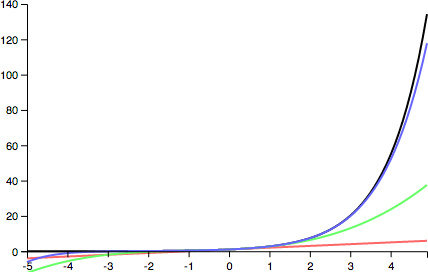
\includegraphics[scale=0.65]{taylor-series-f.png}
\caption{The Taylor polynomial of $f$ plotted for values of $n = 2$ \red{(red)}, $n = 4$ \green{(green)}, and $n = 8$ \blue{(blue)}. $f(x)$ is plotted in black. The $2$-degree Taylor polynomial is equivalent to the tangent line of $f$ at the point $x_0$. As the degree $n$ increases we have better and better approximation of the original function.}
\end{figure}

\[
\begin{aligned}
g(x) = \ln(x+1) &= x - \frac{x^2}{2} + \frac{x^3}{3} - \frac{x^4}{4} + \frac{x^5}{5} - \frac{x^6}{6} + \dots + R_n\left(x\right) \\
&= \sum_{n=1}^\infty (-1)^{n+1} \frac{x^n}{n}
\end{aligned}
\]

\begin{figure}[H]
\centering
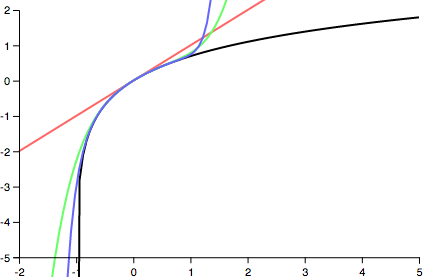
\includegraphics[scale=0.65]{taylor-series-g.png}
\caption{The Taylor polynomial of $g$ plotted for values of $n = 2$ \red{(red)}, $n = 6$ \green{(green)}, and $n = 12$ \blue{(blue)}. $g(x)$ is plotted in black. Once again when $n = 2$ we have the tangent line of $g$ at $x_0$. The Taylor polynomials for $g$ appear to be very accurate close to the center, but diverge quickly outside of this neighborhood.}
\end{figure}

The error for a Taylor polynomial can be bounded by the remainder function.
\[
|f(x) - T_n(x)| \le R_n(x) = e^x \frac{x^{n}}{n!}
\]

\[
|g(x) - T_n(x)| \le R_n(x) = \ln(x+1) (-1)^{n+1} \frac{x^{n}}{n}
\]

Where $T_n(x)$ is the Taylor polynomial for $f$ or $g$ respectively. Here as $n \to \infty$ the $|f(x) - T_n(x)| \to 0$ and $|g(x) - T_n(x)| \to 0$. For small values of $n$ the error is small around to the center point $x_0 = 0$ and grows as we move away from the center.

}

\item \textbf{A ``simple'' program:} Write a program that reads $n$ and the entries $x_1$, $x_2$, $\cdots$, $x_n$ of a vector $x \in \mathbb{R}^n$ from standard input and prints \[||x||_2 = \sqrt{\sum_{i=1}^n x_i^2}\] to standard output.

\begin{minted}[mathescape,
               linenos,
               numbersep=5pt,
               gobble=2,
               framesep=2mm]{clojure}
  (defn norm [x]
    {:pre [(coll? x)]}
    (->> x
         (map #(Math/pow % 2))
         (apply +)
         Math/sqrt))

  ;; Examples
  (norm [1 2 3]) => 3.7416573867739413
  (norm (range 20)) => 49.69909455915671
  (norm [1 1 1]) => 1.7320508075688772
  (norm [1 0 0]) => 1.0
  (norm [3 4]) => 5.0
\end{minted}

{\color{blue}

\textbf{Explanation:} We define a function that takes one argument a vector $x$, and asserts that it is a collection (in this environment any ``collection'' can be treated like a vector) on line 2. We use the thread last operator \textit{->>} to nest the evaluation of each statement through the end of the next function, similar to a composition. We start with $x$ and apply the $x_i^2$ operation to each value in the vector using a $map$ operation, we sum all the elements up, and lastly apply the $sqrt$ operation. The result of this is implicitly set as the return value of the function.

}

\item \textbf{Some Iteration:} Consider the iteration $x_{n+1} = F(x_n) = \sin x_n$, $x_0 = 1$ (where of course the angle is measured in radians). What does our theory tell us about convergence? Show that the iteration does converge! What is the limit? How fast does the iteration converge? \textbf{Carefully explain the effects of rounding errors.}

{\color{blue}

\begin{figure}[H]
\centering
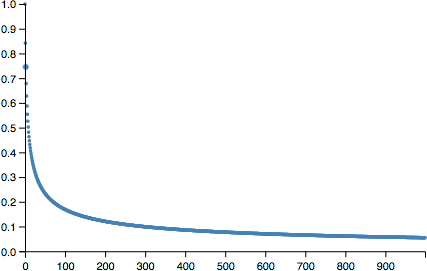
\includegraphics[scale=0.65]{convergence-sinx-double.png}
\caption{The iteration of $F(x_n)$ visually appears to converge.}
\end{figure}

We have the function $F(x_n) = \sin x_n = x_{n+1}$ and we want to know if it converges such that $\sin \alpha = \alpha$ where $\alpha$ is a fixed point of the iteration $F(x_n)$.

We know that a function has a fixed point if it intersects with the identity function $x = y$ in a specified interval. Consider $g(x) = \sin(x) - x = 0$ on the interval $[-1, 1]$. At the left bounds $x = -1$ we have $g(-1) > 0$, and at the right we have $g(1) < 0$, thus by the intermediate value theorem we know that it must have a root in the interval $[-1, 1]$. Therefore there exists a value of $x$ such that $\sin x = x$ within this interval. It's also obvious that $x = 0$ is the fixed point such that $\sin x = x$.

\begin{figure}[H]
\centering
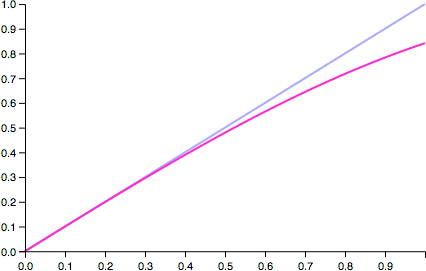
\includegraphics[scale=0.65]{sinx-xy-plot.png}
\caption{$\sin x = y$ crosses the function $x = y$ at $x = 0$, which is a fixed point of $\sin(x)$.}
\end{figure}

The derivative of $\sin^\prime x = \cos x$ is between $[0, 1]$ on the
interval $x \in [0,1]$. So $\sin x$ is a monotone decreasing function
on this interval and we know that it has no other fixed points and
must converge to $0$. Therefore iterating from $x_0 = 1$ will
eventually converge to $0$.

With Newton's method the convergence of $F(x_n)$ is very slow. The
value for the Newton's step $\frac{F(x)}{F^\prime(x)}$ becomes very
small as we move closer to $0$ from above, becuase the rate of change
approaches $1$. This can be seen visually
as the curve for $F(x)$ gets very close to $x = y$ but only touches it
at $x=0$. For example, when coded with double precision, after
$100000$ iterations we arrived at $x=0.00547696985405864$. Successive
iterations would continue to decrease, but would do so slower and slower.
}

\begin{minted}[mathescape,
               linenos,
               numbersep=5pt,
               gobble=2,
               framesep=2mm]{clojure}
  (first (drop 100000 (iterate #(Math/sin %) 1)))
  => 0.00547696985405864
\end{minted}
{\color{blue}

As the iteration converges we will have to deal with very small and
precise numbers. The precision of these numbers will quickly grow
beyond the bounds of traditionaly floating point or double arithmetic
operations. It's possible that trying to converge to $0$ may never
go below a precise threshold, or may skip around $0$ with once the
iteration of $F(x_n)$ becomes arbitrarily small.

}

\item \textbf{Newton's Method:} Suppose $f$ has a root of multiplicity $p>1$ at
$x = \alpha$, i.e. \[f(\alpha) = f^\prime(\alpha) = \dots =
f^{(p-1)}(\alpha) = 0\text{,    }f^{(p)} (\alpha) \ne 0\]. (a) Show
that Newton's method applied to $f(x) = 0$ converges linearly to
$\alpha$. (b) Show that this modification of Newton's
method: \[x_{k+1} = x_k - p \frac{f(x_k)}{f^\prime(x_k)}\] converges
quadratically to $\alpha$. \textbf{Hint:} You probably are thinking of
using L'H\^{o}pital, but the problem is much easier if you think of
$f$ as being defined by $f(x) = (x-\alpha)^p F(x)$ where $F(\alpha)
\ne 0$.

{\color{blue}
% TODO

\begin{enumerate}

\item

We have
\[
g(x) = x - \frac{f(x)}{f^\prime(x)}
\]

Then
\[
g^\prime(x) = \frac{f(x)\, f^{\prime \prime}(x)}{{f^\prime(x)}^2}
\]

If $f(x) = (x-\alpha)^p F(x)$ then we have that
\[
\begin{aligned}
f(x) &= (x - \alpha) g_0(x) \\
f^\prime (x) &= p(x - \alpha)^{p-1} F(x) + (x - \alpha)^p F^\prime (x) \\
&= (x - \alpha)^{p-1} g_1(x) \\
f^{\prime \prime} (x) &= p(p - 1)(x - \alpha)^{p-2} F(x) + 2p (x - \alpha)^{p-1}
F^\prime(x) + (x - \alpha)^p F^{\prime \prime} (x) \\
&= (x - \alpha)^{p-2} g_2(x)
\end{aligned}
\]

where $g_0(x)$, $g_1(x)$, and $g_2(x)$ are the successive iterations of $g(x)$.

We can now plug these into the function for $g^\prime$ as it
approaches $\alpha$
\[
\begin{aligned}
\lim_{x \to \alpha} g^\prime(x) &=
\frac{(x - \alpha) g_0(x) (x - \alpha)^{p-2} g_2(x)}
{\left[(x - \alpha)^{p-1} g_1(x)\right]^2} \\
&= \frac{g_0(x) g_2(x)}{g_1(x)^2} \\
&= \frac{p(p - 1)F(\alpha)^2}{p^2 F(\alpha)^2} \\
&= \frac{p - 1}{p} < 1
\end{aligned}
\]

Meaning that our function will linearly converge to $\alpha$ since
$\frac{p - 1}{p} < 1$.


\item

% part (b)
% #19 - http://www.math.purdue.edu/~shen/ma514/HWsol/HW3.pdf

We define an error term $e_n = x_n - \alpha$, and we have that

We can then expand the Taylor series of $f(x_n)$ and eliminate many of
the initial terms because $f(\alpha) = f^\prime(\alpha) = \dots = f^{(p-1)}(\alpha) = 0$

\[
\begin{aligned}
f(x_n) &= f(\alpha + e_n) \\
&= f(\alpha) + e_n f^\prime (\alpha) + \cdots + \frac{e_n^{(p-1)} f^{(p-1)}(\alpha)}{(p-1)!} + \frac{e_n^p f^{(p)} (\alpha)}{p!}
+ \frac{e_n^{p+1} f^{(p+1)} (\xi_n)}{(p+1)!} \\
\Rightarrow f(x_n) &= \frac{e_n^p f^{(p)}(\alpha)}{p!} + \frac{e_n^{p+1} f^{(p+1)} (\xi_n)}{(p+1)!}
\end{aligned}
\]

We then differntiate $f(x_n)$

\[
\begin{aligned}
f^\prime (x_n) = \frac{e_n^{p-1} f^p (\alpha)}{(p-1)!} + \frac{e_n^p f^{(p+1)} (\eta_n)}{p!}
\end{aligned}
\]

Now if we calculate the next error term in our sequence we can see
that there is quadratic convergence.

\[
\begin{aligned}
e_{n+1} &= x_{n+1} - \alpha \\
&= x_n - \alpha - \frac{p f(x_n)}{f^\prime (x_n)}\\
&= e_n - \frac{\left(
\frac{e_n^p f^{(p)}(\alpha)}{(p-1)!} + \frac{e_n^{p+1} f^{(p+1)}(\xi_n)}{(p+1)(p-1)!}
\right)}{\left(
\frac{e_n^{p-1} f^{(p)}(\alpha)}{(p-1)!} + \frac{e_n^p f^{(p+1)}(\eta_n)}{p!}
\right)} \\
&= e_n^2 \frac{\left(
\frac{f^{(p+1)}(\eta_n)}{p!} - \frac{f^{(p+1)} (\eta_n)}{(p+1)(p-1)!}
\right)}
{\left(
\frac{f^{(p)}(\alpha)}{(p-1)!} +
\frac{e_n f^{(p+1)}(\eta_n)}{p!}
\right)}
\end{aligned}
\]

Since the term $e_{n+1}$ has a leading coefficient $e_n^2$ we know
that it converges quadratically.


\end{enumerate}

}

\item \textbf{Division without division:} Suppose you have a computer or calculator that has no built-in division. Come up with a fixed point iteration that converges to $1/r$ for any given non-zero number $r$, and that only uses addition, subtraction, and multiplication. \textbf{Hint:} Write down an equation satisfied by $1/r$, apply Newton's method to that equation, and then modify Newton's method so that it doesn't use division. Your resulting method should converge of order 2.

{\color{blue}

We can
\[
\begin{aligned}
f(x) &= \frac{1}{r} = x \\
&\Rightarrow 1 = xr \\
&\Rightarrow \frac{1}{x} = r \\
&\Rightarrow \frac{1}{x} - r = 0
\end{aligned}
\]

\[
f^\prime (x) = \frac{-1}{x^2}
\]

\[
\begin{aligned}
F(x) &= x - \frac{f(x)}{f^\prime(x)} \\
&= x - \frac{\frac{1}{x} - r}{\frac{-1}{x^2}} \\
&= x + \left(\frac{1}{x} - r\right) x^2 \\
&= x(2 - xr)
\end{aligned}
\]

}

\begin{minted}[mathescape,
               linenos,
               numbersep=5pt,
               gobble=2,
               frame=lines,
               framesep=2mm]{clojure}
  (defn reciprocal [r]
    (let [convergent? (fn [{:keys [steps error] :or {steps 0
                                                    error 1}}]
                        (or (< (Math/abs (double error)) 0.00001)
                            (> steps 20)))
          next-guess (fn [{:keys [x last steps] :or {last 0
                                                    steps 0}}]
                       (let [guess (* x (- 2 (* x r)))]
                         {:steps (inc steps)
                          :error (- last guess)
                          :last x
                          :x guess}))
          answer (first (drop-while #(not (convergent? %))
                                    (iterate #(next-guess %)
                                             {:x (if (= 20 r) 0.01 0.1)})))]
      (println answer)
      (:x answer)))

  (reciprocal 3) => 0.33333333333333337
  (reciprocal 4) => 0.24999999999999997
\end{minted}

{\color{blue}
\textbf{Explanation: } We define a function that uses a few local
functions to perform Newton's method. On line 2, we locally define the
\texttt{convergent?} function which checks if our answer is below a
threshold or the iteration has exceeded a maximum number of steps. On
line 6, we define a function called \texttt{next-guess} that performs
the actual Newton's step operation $x(2 - xr)$ and returns it's value
with additional metadata to help with iteration. On line 13 we perform
the calculation, starting at a suitably small value and treating our
function \texttt{next-guess} as a sequence of iterations we take only
the first convergent value we receive.
}

\item \textbf{A cubically convergent method:} Consider the iteration \[x_{k+1} = g(x_k)\text{    where    }g(x) = x - \frac{f(x)}{f^\prime(x)} - \frac{1}{2} \frac{f^2 (x) f^{\prime \prime} (x)}{\left(f^\prime(x)\right)^3}\]. (We assume $f$ is sufficiently differentiable, and $f^\prime(x) \ne 0$.) Suppose that $g(\alpha) = \alpha$. Show that \[g^\prime(\alpha) = g^{\prime\prime}(\alpha) = 0\]. (Thus the fixed point method will converge of order at least 3 if we start sufficiently close to $\alpha$.)

{\color{blue}

\[
g(x) = x - \frac{f(x)}{f^\prime(x)} - \frac{{f(x)}^2\, f^{\prime \prime}(x)}{2\, { f^\prime(x)}^3}
\]

\[
\begin{aligned}
g^\prime (x)
%&= 1 - \frac{{f^\prime (x)}^2 - f(x)\, f^{\prime \prime}(x)}{f^\prime(x)^2} - \frac{{f^\prime(x)}^3\, \left({f(x)}^2\, f^{(3)}(x) + f(x)\, f^{\prime \prime}(x)\, f^\prime(x)\, 2\right) - 3\, {f(x)}^2\, {f^\prime(x)}^2\, { f^{\prime \prime}(x)}^2}{{ f^\prime(x)}^6} \\
%&= 1 - \frac{{f^\prime (x)}^2 - f(x)\, f^{\prime \prime}(x)}{f^\prime(x)^2} -\frac{{f(x)}^2\, f^{(3)}(x)\, f^\prime(x) - 3\, {f(x)}^2\, { f^{\prime \prime}(x)}^2 + 2\, f(x)\, { f^\prime(x)}^2\, f^{\prime \prime}(x)}{{ f^\prime(x)}^4} \\
%&= 1 - 1 - \frac{f(x)\, f^{\prime \prime}(x)}{f^\prime(x)^2}
%-\frac{{f(x)}^2\, f^{(3)}(x)\, f^\prime(x) - 3\, {f(x)}^2\, { f^{\prime \prime}(x)}^2 + 2\, f(x)\, { f^\prime(x)}^2\, f^{\prime \prime}(x)}{{ f^\prime(x)}^4} \\
&= \frac{3\, {f(x)}^2\, { f^{\prime \prime}(x)}^2}{2\, { f^\prime(x)}^4} - \frac{{f(x)}^2\, f^{(3)}(x)}{2\, { f^\prime(x)}^3} \\
\end{aligned}
\]

\[
\begin{aligned}
g^\prime (\alpha) &= \frac{3\, {f(\alpha)}^2\, { f^{\prime \prime}(\alpha)}^2}{2\, { f^\prime(\alpha)}^4} - \frac{{f(\alpha)}^2\, f^{(3)}(\alpha)}{2\, { f^\prime(\alpha)}^3} \\
&= \frac{3\, {(0)}^2\, { f^{\prime \prime}(\alpha)}^2}{2\, { f^\prime(\alpha)}^4} - \frac{{(0)}^2\, f^{(3)}(\alpha)}{2\, { f^\prime(\alpha)}^3} \\
&= \frac{0}{2\, { f^\prime(\alpha)}^4} - \frac{0}{2\, { f^\prime(\alpha)}^3} \\
&= 0
\end{aligned}
\]

Likewise when differentiating $g^\prime(x)$ we will have a function
that is $0$ when $x = \alpha$ since $f(\alpha) = 0$,

\[
\begin{aligned}
g^{\prime \prime} (x) &= \frac{3\, f(x)\, {f^{\prime \prime}(x)}^2}{{ f^\prime(x)}^3} -
\frac{6\, {f(x)}^2\, {f^{\prime \prime}(x)}^3}{{ f^\prime(x)}^5} -
\frac{{f(x)}^2\,  f^{(4)}(x)}{2\, { f^\prime(x)}^3} - \frac{f(x)\,
  f^{(3)}(x)}{{ f^\prime(x)}^2} + \frac{9\, {f(x)}^2\,  f^{(3)}(x)\,
   f^{\prime \prime}(x)}{2\, { f^\prime(x)}^4} \\
g^{\prime \prime} (\alpha) &= 0
\end{aligned}
\]

}

\item \textbf{Polynomial Interpolation:}
Suppose you want to interpolate to the data
$(x_i, y_i)$, $i=0,\dots,n$ by a polynomial of degree $n$. Recall that
the interpolating polynomial $p$ can be written in its Lagrange form
as
\[
p(x) = \sum_{i=0}^n y_i L_i(x)\text{    where    } L_i(x) =
\frac{\prod_{i\ne j} (x - x_j)}{\prod_{i \ne j} (x_i - x_j)}.
\]
Show that
\[\sum_{i=0}^n x_i^j L_i(x) = x^j\text{    for    } j=0,\dots,n.\]

{\color{blue}
If $y_i = x_i^j$ then we have,

\[
\begin{aligned}
p(x) &= \sum_{i=0}^n x_i^j L_i(x) \\
&= \sum_{i=0}^n x_i^j \frac{\prod_{i\ne j} (x - x_j)}{\prod_{i \ne j}
  (x_i - x_j)} \\
&= \sum_{i=0}^n x_i^j
\frac{(x - x_0)(x - x_1)\cdots (x - x_{j-1})(x - x_{j+1}) \cdots (x - x_n)}
{(x_i - x_0)(x_i - x_1)\cdots (x_i - x_{j-1})(x_i - x_{j+1}) \cdots (x_i - x_n)} \\
&= \sum_{i=0}^n x_i^j
\frac{(x - x_0)(x - x_1)\cdots (x - x_{j-1})(x - x_{j+1}) \cdots (x - x_n)}
{(x_i - x_0)(x_i - x_1)\cdots (x_i - x_{j-1})(x_i - x_{j+1}) \cdots
  (x_i - x_n)}
\frac{(x_i - x_j)}{(x_i - x_j)} \\
&= \sum_{i=0}^n
\frac{(x_i^{j+1} - x_i^j x_j)(x - x_0)(x - x_1)\cdots (x - x_{j-1})(x - x_{j+1}) \cdots (x - x_n)}
{n (x_i - x_j)(x_i - x_0)(x_i - x_1)\cdots (x_i - x_{j-1})(x_i - x_{j+1}) \cdots
  (x_i - x_n)} \\
&= \sum_{i=0}^n
\frac{x^j (x_i - x_j)(x_i - x_0)(x_i - x_1)\cdots (x_i - x_{j-1})(x_i - x_{j+1}) \cdots
  (x - x_n)}
{n (x_i - x_j)(x_i - x_0)(x_i - x_1)\cdots (x_i - x_{j-1})(x_i - x_{j+1}) \cdots
  (x_i - x_n)} \\
&= x^j \sum_{i=0}^n
\frac{(x_i - x_j)(x_i - x_0)(x_i - x_1)\cdots (x_i - x_{j-1})(x_i - x_{j+1}) \cdots
  (x - x_n)}
{n (x_i - x_j)(x_i - x_0)(x_i - x_1)\cdots (x_i - x_{j-1})(x_i - x_{j+1}) \cdots
  (x_i - x_n)} \\
&= x^j \sum_{i=0}^n
\frac{1} {n} \\
&= x^j
\end{aligned}
\]


}

\item \textbf{Uniqueness of the interpolating polynomial:} Assume you are
given the data
\[\begin{aligned}
x_i\;&: \,\, 1 \,\, 2 \,\, 4 \,\, 8 \\
y_i\;&: \,\, 1 \,\, 2 \,\, 3 \,\, 4
\end{aligned}\] Construct the interpolating polynomial using

\begin{enumerate}
\item the power form
\item the Lagrange form
\item the Newton form,
\end{enumerate}
and show that they all yield the same polynomial.

{\color{blue}

\begin{enumerate}
\item[(a) the power form]

\[
\begin{aligned}
  p(x) &= a_0 + a_1 x + a_2 x^2 + a_3 x^3 \\
  \Rightarrow p(x) &= V_n \vect{a} = \vect{y} \\
p(x) &=
\left(\begin{array}{cccc}
  1 & x_0 & x_0^2 & x_0^3 \\
  1 & x_1 & x_1^2 & x_1^3 \\
  1 & x_2 & x_2^2 & x_2^3 \\
  1 & x_3 & x_3^2 & x_3^3
\end{array}\right)
\left(\begin{array}{c}
  a_0 \\
  a_1 \\
  a_2 \\
  a_3
\end{array}\right)
= \left(\begin{array}{c}
  y_0 \\
  y_1 \\
  y_2 \\
  y_3
\end{array}\right) \\
p(x) &= \left(\begin{array}{cccc}
  1 & 1 & 1 & 1 \\
  1 & 2 & 4 & 8 \\
  1 & 4 & 16 & 64 \\
  1 & 8 & 64 & 512
\end{array}\right)
\left(\begin{array}{c}
  a_0 \\
  a_1 \\
  a_2 \\
  a_3
\end{array}\right)
= \left(\begin{array}{c}
  1 \\
  2 \\
  3 \\
  4
\end{array}\right) \\
p(x) &= \left(\begin{array}{cccc}
  1 & 1 & 1 & 1 \\
  1 & 2 & 4 & 8 \\
  1 & 4 & 16 & 64 \\
  1 & 8 & 64 & 512
\end{array}\right)
\left(\begin{array}{c}
  - \frac{10}{21}\\
  \frac{7}{4}\\
  - \frac{7}{24}\\
  \frac{1}{56}
\end{array}\right)
= \left(\begin{array}{c}
  1 \\
  2 \\
  3 \\
  4
\end{array}\right) \\
p(x) &= \frac{1}{56} x^3 - \frac{7}{24} x^2 + \frac{7}{4} x - \frac{10}{21}
\end{aligned}
\]

\item[(b) the Lagrange form]

\[
L(x) = \frac{\prod_{i \ne j} (x - x_j)}{\prod_{i \ne j} (x_i - x_j)}
\]

\[
\begin{aligned}
  p(x) &= \sum_{i=0}^n y_i L(x) \\
  p(x) &= 1 \frac{(x-2)(x-4)(x-8)}{(1-2)(1-4)(1-8)} + 2 \frac{(x-1)(x-4)(x-8)}{(2-1)(2-4)(2-8)} \\
  &    + 3 \frac{(x-1)(x-2)(x-8)}{(4-1)(4-2)(4-8)} + 4 \frac{(x-1)(x-2)(x-4)}{(8-1)(8-2)(8-4)}\\
  p(x) &= \frac{x^3 - 14\, x^2 + 56\, x - 64}{-21} + \frac{x^3 - 13\, x^2 + 44\, x - 32}{12} \\
&    + \frac{x^3 - 11\, x^2 + 26\, x - 16}{-24} + \frac{x^3 - 7\, x^2 + 14\, x - 8}{168} \\
p(x) &= \frac{1}{56} x^3 - \frac{7}{24} x^2 + \frac{7}{4} x - \frac{10}{21}
\end{aligned}
\]

\item[(c) the Newton form]

\[
\begin{aligned}
p_k(x) &= \sum_{i=0}^k c_i \prod_{j=0}^{i-1} (x - x_j) \\
\Rightarrow p_0(x) &= c_0 \\
p_1(x) &= p_0(x) + c_1(x -x_0) \\
p_2(x) &= p_1(x) + c_2(x -x_0)(x - x_1) \\
p_3(x) &= p_2(x) + c_3(x -x_0)(x - x_1)(x - x_2) \\
\Rightarrow p_0(x) &= y_0 \\
p_1(x) &= p_0(x) + \frac{y_1 - P_0(x_1)}{(x_1 - x_0)} (x -x_0) \\
p_2(x) &= p_1(x) + \frac{y_2 - P_1(x_2)}{(x_2 - x_0)(x_2 - x_1)} (x -x_0)(x - x_1) \\
p_3(x) &= p_2(x) + \frac{y_3 - P_2(x_3)}{(x_3 - x_0)(x_3 - x_1)(x_3 - x_2)} (x -x_0)(x - x_1)(x - x_2) \\
\Rightarrow p_0(x) &= 1 \\
p_1(x) &= p_0(x) + \frac{2 - P_0(2)}{(2 - 1)} (x -1) \\
p_2(x) &= p_1(x) + \frac{3 - P_1(4)}{(4 - 1)(4 - 2)} (x -1)(x - 2) \\
p_3(x) &= p_2(x) + \frac{4 - P_2(8)}{(8 - 1)(8 - 2)(8 - 4)} (x -1)(x - 2)(x - 4) \\
\end{aligned}
\]
\[
\begin{aligned}
\Rightarrow p_0(x) &= 1 \\
p_1(x) &= 1 + \frac{2 - 1}{(2 - 1)} (x -1) \\
&= 1 + \frac{1}{1} (x - 1) \\
&= x \\
p_2(x) &= x + \frac{3 - 4}{(4 - 1)(4 - 2)} (x -1)(x - 2) \\
&= x - \frac{1}{6} (x - 1) (x - 2) \\
&= x - \frac{x^2 - 3x + 2}{6} \\
&= - \frac{x^2}{6} + \frac{3\, x}{2} - \frac{1}{3} \\
p_3(x) &= - \frac{x^2}{6} + \frac{3\, x}{2} - \frac{1}{3} + \frac{4 - 1}{(8 - 1)(8 - 2)(8 - 4)} (x -1)(x - 2)(x - 4) \\
&= - \frac{x^2}{6} + \frac{3\, x}{2} - \frac{1}{3} + \frac{3}{168} (x -1)(x-2)(x-4) \\
&= - \frac{x^2}{6} + \frac{3\, x}{2} - \frac{1}{3} + \frac{3}{168} \left(x^3 - 7\, x^2 + 14\, x - 8\right) \\
&= - \frac{x^2}{6} + \frac{3\, x}{2} - \frac{1}{3} + \frac{3\, x^3 - 21\, x^2 + 42\, x - 24}{168} \\
&= \frac{1}{56} x^3 - \frac{7}{24} x^2 + \frac{7}{4} x - \frac{10}{21} \\
\Rightarrow P(x) &= \frac{1}{56} x^3 - \frac{7}{24} x^2 + \frac{7}{4} x - \frac{10}{21}
\end{aligned}
\]

\end{enumerate}

}

\item \textbf{The infamous Runge-Phenomenon:} It is not generally true that higher degree interpolation polynomials yield more accurate approximations. This is illustrated in this problem. Let \[f(x) = \frac{1}{1+x^2}\text{    and    }x_j = -5 + jh\text{,    }j=0,1,\dots,n\text{,    }h = \frac{10}{n}.\] For \[n=1,2,3,\dots,20\] plot the graph (in the interval $[-5,5]$) of the interpolant \[p(x) = \sum_{i=0}^n \alpha_i x^i\] defined by \[p(x_i) = f(x_i)\text{,    }i=0,1,\dots,n.\]

{\color{blue}

\begin{figure}[H]
\centering
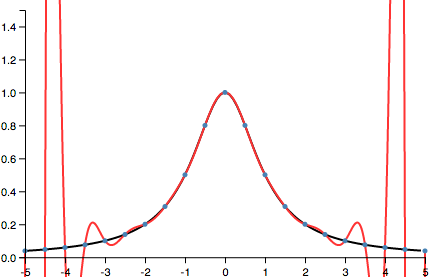
\includegraphics[scale=0.65]{runge-equidistant.png}
\caption{We interpolate points obtained from the Runge function across
  an equidistant interval with $n=20$ in red. The original Runge
  function is plotted in black, along with the points we've
  interpolated from. The interpolated polynomial fluctuates wildly at
  either end of our domain.}
\end{figure}

\begin{figure}[H]
\centering
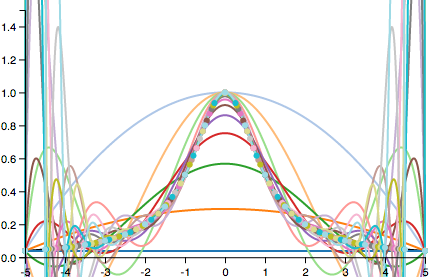
\includegraphics[scale=0.65]{runge-equidistant-n-1-20.png}
\caption{Interpolating several functions for $n = 1,\dots,20$}
\end{figure}

We can see that as we interpolate more points the center of our
function gets approximated better, but the end points become more
unstable. They fluctuate greatly trying to interpolate all points on
the interval.

}

\item \textbf{Judicious interpolation:} Repeat the above except that you interpolate at the roots of the Chebycheff polynomials, i.e. \[x_i = 5 \cos \frac{i \pi}{n},\;\;\; i=0,1,\dots,n.\]

{\color{blue}

\begin{figure}[H]
\centering
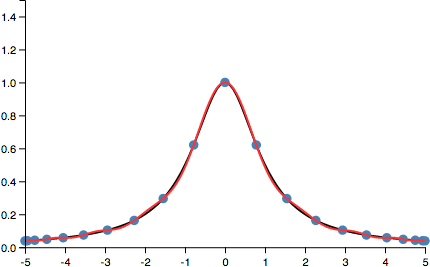
\includegraphics[scale=0.65]{runge-chebycheff.png}
\caption{We interpolate points obtained from the Runge function across
  an interval of points with $n=20$ made up from the Chebycheff roots
  in red. The original Runge function is plotted in black, along with
  the points we've interpolated from. Some minor fluctuation is
  visible, however it's overall much more accurate in our domain.}
\end{figure}

\begin{figure}[H]
\centering
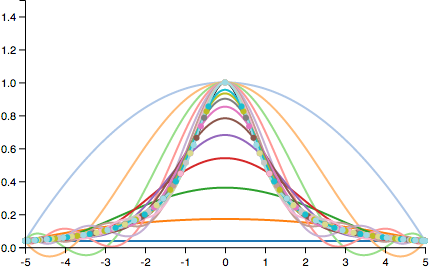
\includegraphics[scale=0.65]{runge-chebycheff-n-1-20.png}
\caption{Once again plotting several interpolations with
  $n=1,\dots,20$ we can see that all the functions interpolated with
  the Chebycheff roots behave much better than the previous problem
  with equidistant points.}
\end{figure}

Here we have that our interpolated polynomial still fluctuates near
the boundaries of our interpolation, but it behaves much better as the
points are distributed more at either end, and thus interpolated better.

}

\item \textbf{Least Squares approximation of functions:} Find a linear function $l(x)$ such that \[\int_0^1 (\mathrm{e}^x - l(x))^2 \text{d}x = \min.\]

{\color{blue}

\[
f = {\left(\mathrm{e}^{x} - a\, x - b\right)}^2
\]

\[
\nabla f =
\left(\begin{array}{c} 2\, x\, \left(\mathrm{e}^{x} - a\, x - b\right)\\ 2\, b - 2\, \mathrm{e}^{x} + 2\, a\, x \end{array}\right)
\]

\[
\int_0^1 \nabla f \text{d}x =
\left(\begin{array}{c} \frac{2\, a}{3} + b - 2\\ a + 2\, b - 2\, \mathrm{e} + 2 \end{array}\right)
\]

\[
\Rightarrow a = 18 - 6\, \mathrm{e},\,\, b = 4\, \mathrm{e} - 10
\]

\[
\begin{aligned}
\Rightarrow l(x) &= (18 - 6 \, \mathrm{e}) x + (4 \, \mathrm{e} - 10)
\end{aligned}
\]

}

\item \textbf{An alternative approximation problem:}
Find a linear function $l(x)$ such that
\[
\int_0^1 |\mathrm{e}^x - l(x)| \text{d}x = \min.
\]

{\color{blue}

\[
\begin{aligned}
\min &= \int_0^1 |\mathrm{e}^x - a\, x - b| \,\text{d}x \\
&= \int_0^c \mathrm{e}^x - a\, x - b \,\text{d}x +
\int_c^d -\mathrm{e}^x + a\, x + b \,\text{d}x +
\int_d^1 \mathrm{e}^x - a\, x - b \,\text{d}x
\end{aligned}
\]

\[
\begin{aligned}
f &= \mathrm{e}^x - a\, x - b \\
g &= -\mathrm{e}^x + a\, x + b
\end{aligned}
\]

\[
\begin{aligned}
\nabla f = \left(\begin{array}{c} - x\\ -1 \end{array}\right), \,\,
\nabla g = \left(\begin{array}{c} x\\ 1 \end{array}\right)
\end{aligned}
\]

\[
\begin{aligned}
 \int_0^c \nabla f \text{d}x +
\int_c^d \nabla g \text{d}x +
\int_d^1 \nabla f \text{d}x
&= \left(\begin{array}{c} - \frac{c^2}{2}\\ - c \end{array}\right) +
\left(\begin{array}{c} \frac{d^2}{2} - \frac{c^2}{2}\\ d -
  c \end{array}\right) +
\left(\begin{array}{c} \frac{d^2}{2} - \frac{1}{2}\\ d -
  1 \end{array}\right) \\
&= \left(\begin{array}{c}  - c^2 + d^2 - \frac{1}{2}\\ 2\, d - 2\, c - 1 \end{array}\right)
\end{aligned}
\]

\[
\begin{aligned}
\Rightarrow c = \frac{1}{4},\,\, d = \frac{3}{4}
\end{aligned}
\]

\[
\begin{aligned}
&\Rightarrow
\left(\begin{array}{c}
a\, c + b = e^c \\
a\, d + b = e^d
\end{array}\right) \\
&= \left(\begin{array}{c}
\frac{a}{4} + b = \mathrm{e}^{\frac{1}{4}}\\
\frac{3\, a}{4} + b = \mathrm{e}^{\frac{3}{4}}
\end{array}\right)
\end{aligned}
\]

\[
a = 2\, \mathrm{e}^{\frac{3}{4}} - 2\, \mathrm{e}^{\frac{1}{4}},b = \frac{3\, \mathrm{e}^{\frac{1}{4}}}{2} - \frac{\mathrm{e}^{\frac{3}{4}}}{2}
\]

\[
l(x) =
\left(2\, \mathrm{e}^{\frac{3}{4}} - 2\, \mathrm{e}^{\frac{1}{4}}\right) x +
\frac{3\, \mathrm{e}^{\frac{1}{4}}}{2} - \frac{\mathrm{e}^{\frac{3}{4}}}{2}
\]

}

\item \textbf{Another alternative approximation problem:} Find a linear function $l(x)$ such that \[\max_{0\le x\le 1} |\mathrm{e}^x - l(x)| = \min.\]

{\color{blue}

We find the values for $f(x) = \mathrm{e}^x - a\, x - b$ where the
difference is large.

\[
\begin{aligned}
f(x) &= |\mathrm{e}^x - a\, x - b| \\
f(0) &= | 1 - b | \\
f(1) &= | \mathrm{e} - a - b| \\
f(\log a) &= | \mathrm{e}^{\log a} - a\, \log a - b| \\
&= | a - a\, \log a - b |
\end{aligned}
\]

By setting these equations equal to each other, we can eliminate
variables, and find the values for $a$ and $b$ that minimize $f(x)$.

\[
\begin{aligned}
1 - b &= \mathrm{e} - a - b \\
\Rightarrow a &= \mathrm{e} - 1
\end{aligned}
\]

\[
\begin{aligned}
b - 1 &= a - a \log a - b \\
2b &= 1 + a - a \log a \\
&= 1 + (\mathrm{e} - 1) - (\mathrm{e} -1) \log (\mathrm{e} - 1) \\
&= \mathrm{e} - (\mathrm{e} -1) \log (\mathrm{e} - 1) \\
\Rightarrow b &=
\frac{\mathrm{e} - (\mathrm{e} -1) \log (\mathrm{e} - 1)}{2} \\
\end{aligned}
\]

\[
l(x) =
\left(\mathrm{e} - 1\right)\, x +
\frac{\mathrm{e} - (\mathrm{e} -1) \log (\mathrm{e} - 1)}{2} \\
\]

\begin{figure}[H]
\centering
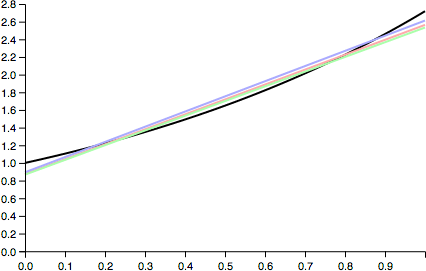
\includegraphics[scale=0.65]{approximations-of-e-x.png}
\caption{We plot $e^x$ in black, with the solutions to exercises 11 (red),
12 (green), and 13 (blue). We can visually see that our solutions all
linearly approximate $e^x$ on $[0,1]$.}
\end{figure}

}


\end{enumerate}

\end{document}
